\subsection{Testing for Weak SSL/TSL Ciphers, Insufficient Transport Layer Protection - OTG-CRYPST-001}
\subsubsection{BANK-APP}
\begin{longtable}[l]{ p{2.3cm} | p{.79\linewidth} }\hline
    & \textbf{BANK-APP}
    \\ \hline
    \textbf{Observation} & It has been found that application works only on HTTP and does not support transmission over HTTPS. Neither does the application encrypt data used in requests. It is also observed that there are no ports having SSL services and hence no further testing could be done. \\
    \textbf{Discovery} &
     	Tests to determine transmission over HTTP/HTTPS have been described in section \ref{OTG-AUTHN-001}.
     	We also performed tests to check for Basic Authentication over HTTP and SSL configuration in the ports. Following are the details.
     	\begin{itemize}
     	\item \textbf{Test for HTTP Basic Authentication -}
     		\begin{itemize}
	     		\item Open the Login page in the browser. Also open Firebug in Firefox or Developer Tools in Chrome and navigate to the Network tab.
               	\item Enter credentials in the login form and click on "Submit".
                \item Observe the request captured in the Network tab. The response does not contain the \enquote{WWW-Authenticate} header indicating that the server does not use Basic Authentication.
     		\end{itemize}

     	\item \textbf{Test for SSL services -}
     		\begin{itemize}
     			\item Open the terminal and type \code{nmap -sV --reason -PN -n --top-ports 100 <IP-address>}.
     			\item To also check typical ports with SSL support, type \code{nmap --script ssl-cert,ssl-enum-ciphers -p 443,465,993,995 <IP-address>}. See Figure \ref{nmap_ssl_ports}. Observing the output, it can be concluded that none of the ports on the virtual machine support SSL service.
     		\end{itemize}
		\end{itemize}
    \\
    \textbf{Likelihood} & N/A \\
    \textbf{Impact} & N/A \\
    \textbf{Recommen\-dations} & N/A \\ \hline
    \textbf{CVSS} & N/A
    \\ \hline
\end{longtable}

\subsubsection{SecureBank}
\begin{longtable}[l]{ p{2.3cm} | p{.79\linewidth} }\hline
    & \textbf{SecureBank}
    \\ \hline
    \textbf{Observation} & It has been found that application works only on HTTP and does not support transmission over HTTPS. Neither does the application encrypt data used in requests. It is also observed that there are no ports having SSL services and hence no further testing could be done. \\
    \textbf{Discovery} & Same as observed for BANK-APP. \\
    \textbf{Likelihood} & N/A \\
    \textbf{Impact} & N/A \\
    \textbf{Recommen\-dations} & N/A \\ \hline
    \textbf{CVSS} & N/A
    \\ \hline
\end{longtable}

\begin{figure}[ht]
	\centering
	\begin{subfigure}{.45\textwidth}
		\centering
		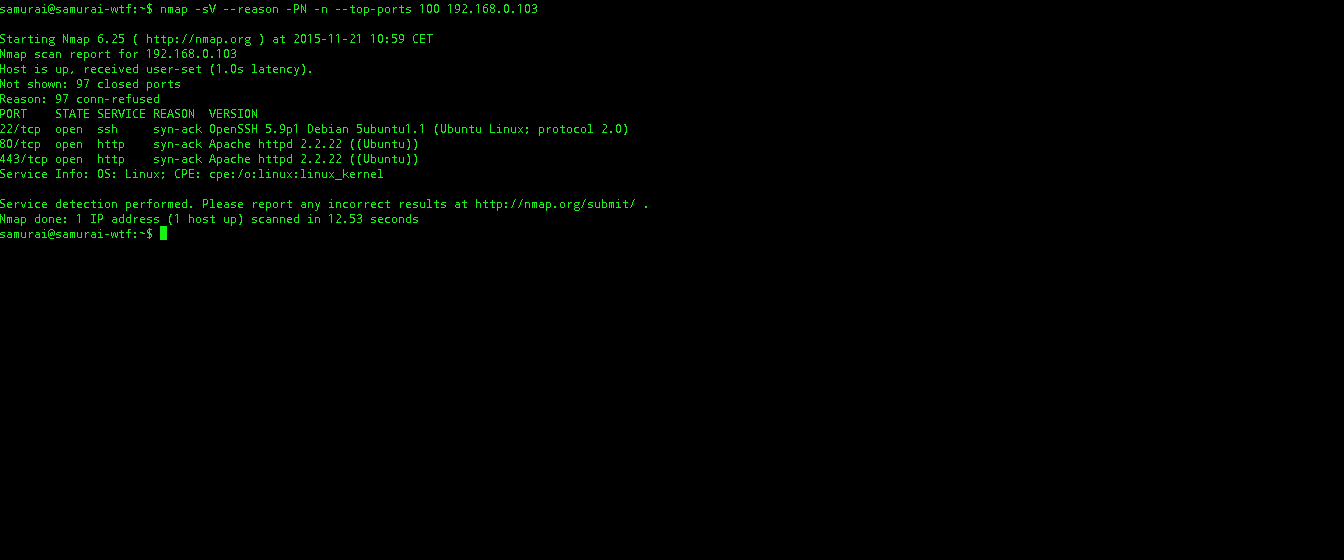
\includegraphics[width=.9\linewidth]{figures/OTG-CRYPST-001_1.png}
		\caption{Nmap - Generic check for ports with SSL support}
	\end{subfigure}\hfill%
	\begin{subfigure}{.45\textwidth}
		\centering
		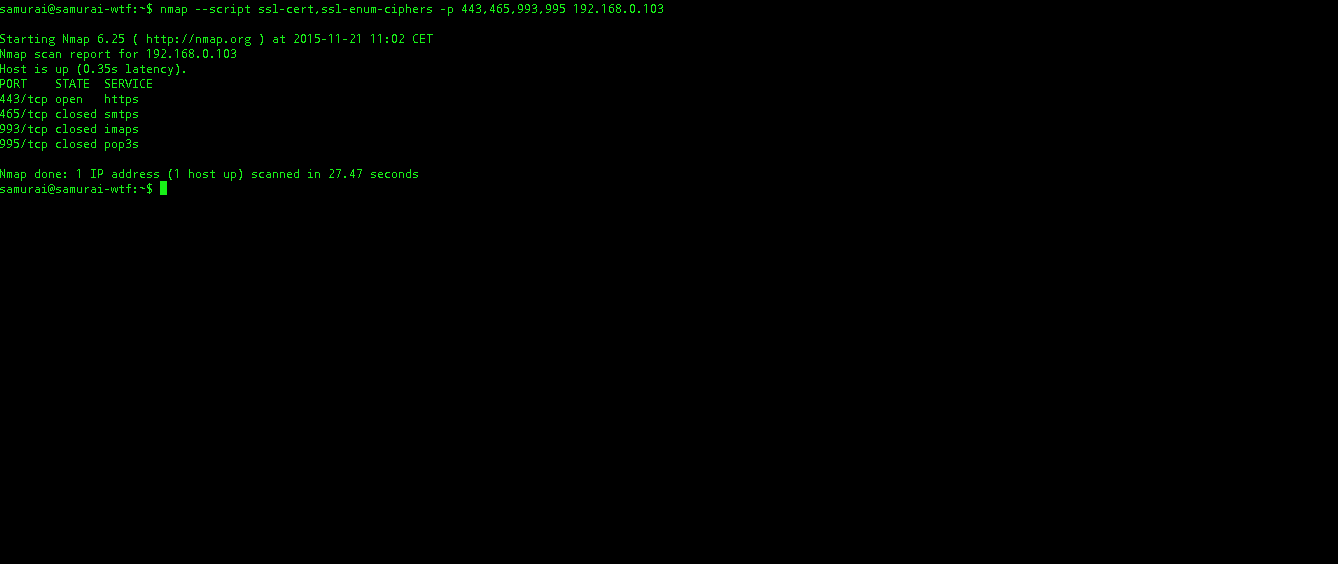
\includegraphics[width=.9\linewidth]{figures/OTG-CRYPST-001_2.png}
		\caption{Nmap - Check for typical ports with SSL configuration}
	\end{subfigure}
	\caption{Testing for ports with SSL configuration}
	\label{fig:nmap_ssl_ports}
\end{figure}

\subsubsection{Comparison}
Both applications are similar in behavior and neither support Basic Authentication or SSL technologies.
\clearpage
